\documentclass[]{tufte-handout}

% ams
\usepackage{amssymb,amsmath}

\usepackage{ifxetex,ifluatex}
\usepackage{fixltx2e} % provides \textsubscript
\ifnum 0\ifxetex 1\fi\ifluatex 1\fi=0 % if pdftex
  \usepackage[T1]{fontenc}
  \usepackage[utf8]{inputenc}
\else % if luatex or xelatex
  \makeatletter
  \@ifpackageloaded{fontspec}{}{\usepackage{fontspec}}
  \makeatother
  \defaultfontfeatures{Ligatures=TeX,Scale=MatchLowercase}
  \makeatletter
  \@ifpackageloaded{soul}{
     \renewcommand\allcapsspacing[1]{{\addfontfeature{LetterSpace=15}#1}}
     \renewcommand\smallcapsspacing[1]{{\addfontfeature{LetterSpace=10}#1}}
   }{}
  \makeatother

\fi

% graphix
\usepackage{graphicx}
\setkeys{Gin}{width=\linewidth,totalheight=\textheight,keepaspectratio}

% booktabs
\usepackage{booktabs}

% url
\usepackage{url}

% hyperref
\usepackage{hyperref}

% units.
\usepackage{units}


\setcounter{secnumdepth}{-1}

% citations
\usepackage{natbib}
\bibliographystyle{plainnat}


% pandoc syntax highlighting
\usepackage{color}
\usepackage{fancyvrb}
\newcommand{\VerbBar}{|}
\newcommand{\VERB}{\Verb[commandchars=\\\{\}]}
\DefineVerbatimEnvironment{Highlighting}{Verbatim}{commandchars=\\\{\}}
% Add ',fontsize=\small' for more characters per line
\newenvironment{Shaded}{}{}
\newcommand{\AlertTok}[1]{\textcolor[rgb]{1.00,0.00,0.00}{\textbf{#1}}}
\newcommand{\AnnotationTok}[1]{\textcolor[rgb]{0.38,0.63,0.69}{\textbf{\textit{#1}}}}
\newcommand{\AttributeTok}[1]{\textcolor[rgb]{0.49,0.56,0.16}{#1}}
\newcommand{\BaseNTok}[1]{\textcolor[rgb]{0.25,0.63,0.44}{#1}}
\newcommand{\BuiltInTok}[1]{#1}
\newcommand{\CharTok}[1]{\textcolor[rgb]{0.25,0.44,0.63}{#1}}
\newcommand{\CommentTok}[1]{\textcolor[rgb]{0.38,0.63,0.69}{\textit{#1}}}
\newcommand{\CommentVarTok}[1]{\textcolor[rgb]{0.38,0.63,0.69}{\textbf{\textit{#1}}}}
\newcommand{\ConstantTok}[1]{\textcolor[rgb]{0.53,0.00,0.00}{#1}}
\newcommand{\ControlFlowTok}[1]{\textcolor[rgb]{0.00,0.44,0.13}{\textbf{#1}}}
\newcommand{\DataTypeTok}[1]{\textcolor[rgb]{0.56,0.13,0.00}{#1}}
\newcommand{\DecValTok}[1]{\textcolor[rgb]{0.25,0.63,0.44}{#1}}
\newcommand{\DocumentationTok}[1]{\textcolor[rgb]{0.73,0.13,0.13}{\textit{#1}}}
\newcommand{\ErrorTok}[1]{\textcolor[rgb]{1.00,0.00,0.00}{\textbf{#1}}}
\newcommand{\ExtensionTok}[1]{#1}
\newcommand{\FloatTok}[1]{\textcolor[rgb]{0.25,0.63,0.44}{#1}}
\newcommand{\FunctionTok}[1]{\textcolor[rgb]{0.02,0.16,0.49}{#1}}
\newcommand{\ImportTok}[1]{#1}
\newcommand{\InformationTok}[1]{\textcolor[rgb]{0.38,0.63,0.69}{\textbf{\textit{#1}}}}
\newcommand{\KeywordTok}[1]{\textcolor[rgb]{0.00,0.44,0.13}{\textbf{#1}}}
\newcommand{\NormalTok}[1]{#1}
\newcommand{\OperatorTok}[1]{\textcolor[rgb]{0.40,0.40,0.40}{#1}}
\newcommand{\OtherTok}[1]{\textcolor[rgb]{0.00,0.44,0.13}{#1}}
\newcommand{\PreprocessorTok}[1]{\textcolor[rgb]{0.74,0.48,0.00}{#1}}
\newcommand{\RegionMarkerTok}[1]{#1}
\newcommand{\SpecialCharTok}[1]{\textcolor[rgb]{0.25,0.44,0.63}{#1}}
\newcommand{\SpecialStringTok}[1]{\textcolor[rgb]{0.73,0.40,0.53}{#1}}
\newcommand{\StringTok}[1]{\textcolor[rgb]{0.25,0.44,0.63}{#1}}
\newcommand{\VariableTok}[1]{\textcolor[rgb]{0.10,0.09,0.49}{#1}}
\newcommand{\VerbatimStringTok}[1]{\textcolor[rgb]{0.25,0.44,0.63}{#1}}
\newcommand{\WarningTok}[1]{\textcolor[rgb]{0.38,0.63,0.69}{\textbf{\textit{#1}}}}

% longtable

% multiplecol
\usepackage{multicol}

% strikeout
\usepackage[normalem]{ulem}

% morefloats
\usepackage{morefloats}


% tightlist macro required by pandoc >= 1.14
\providecommand{\tightlist}{%
  \setlength{\itemsep}{0pt}\setlength{\parskip}{0pt}}

% title / author / date
\title[正規分布表を求める]{正規分布表を求める}
\author{Sampo Suzuki, CC 4.0 BY-NC-SA}
\date{2021-05-30}

% --- 参考資料 ----------------------------------------------------------------
% https://github.com/Gedevan-Aleksizde/Japan.R2019/blob/master/latex/preamble.tex
% https://teastat.blogspot.com/2019/01/bookdown.html

% --- Packages ----------------------------------------------------------------
% 日本語とtufte, kableExtraを使うために必要なTeXパッケージ指定
% tufteではA4サイズの指定が不可能
%  A4 210mm x 297mm
%   \usepackage[a4paper, total={6.5in, 9.5in}]{geometry}
%   \usepackage{indentfirst}   # tinytexのリポジトリには存在しない?
% \usepackage[a4paper, total={160mm, 247mm}, left=25mm, top=25mm]{geometry}
% \usepackage[pdfbox,tombo]{gentombow}  % トンボを設定する場合は有効にする
% \usepackage{ifthen}                     % 条件分岐用 \ifthenelse{条件}{T}{F}
\usepackage{booktabs}                   % ここからkableExtra用パッケージ
\usepackage{longtable}                  % 
\usepackage{array}                      % 
\usepackage{multirow}                   % 
\usepackage{wrapfig}                    % 
\usepackage{float}                      % 
\usepackage{colortbl}                   % 
\usepackage{pdflscape}                  % 
\usepackage{tabu}                       % 
\usepackage{threeparttable}             % 
\usepackage{threeparttablex}            % 
\usepackage[normalem]{ulem}             % 
\usepackage{inputenc}                   % 
\usepackage{makecell}                   % 
\usepackage{xcolor}                     % ここまでkableExtra用
\usepackage{amsmath}                    % 
\usepackage{fontawesome5}               % fontawesomeを使うために必要
\usepackage{subfig}
\usepackage{xeCJK}                      % 以下、日本語フォント用に必要
\usepackage[noto]{zxjafont}             % Linux環境ではこちを指定
% \usepackage[haranoaji]{zxjafont}      % Windows環境ではこちらを指定する
\usepackage{zxjatype}
\usepackage{pxrubrica}                  % ルビ用
\usepackage{hyperref}                   % ハイパーリンク用必要?

% --- Index ------------------------------------------------------------------
% https://texwiki.texjp.org/?%E7%B4%A2%E5%BC%95%E4%BD%9C%E6%88%90
% これを指定するとIndex(索引)は作成されるが参照ページがズレる
% 中間ファイルの.indではページはズレていないので、その後の結合処理がおかしい
% \usepackage{makeidx}
% \makeindex
% \usepackage{showidx}                  % 索引確認用

% --- Table of Contentes ------------------------------------------------------
% TOCにLOT(List of Tables), LOF(List of Figures), Bibliography, Indexを表示
% \usepackage[nottoc]{tocbibind}

% --- Fonts -------------------------------------------------------------------
% フォントしては index.html でも可能(pandoc用オプションは index.htmlにて)
% \setCJKmonofont{Source Han Code JP}
\setmonofont{Source Han Code JP}
% \setjamonofont{Source Han Code JP}

% ## 日本語フォントの扱いについてはzxjafontパッケージの解説を参照のこと
% # https://mirror.las.iastate.edu/tex-archive/language/japanese/zxjafont/zxjafont.pdf
% #
% ## Windows環境ではなぜかNotoフォントが認識されないので源ノシリーズベースの
% ## 原ノ味フォントかIPAexフォントを利用する(原ノ味はtlmgrでインストール可)
% # \usepackage[haranoaji]{zxjafont}
% # \usepackage[ipaex]{zxjafont}
% #
% ## Windows環境でNotoフォントを指定したい場合は以下のようにheader-includeで
% ## 個別に指定する(setCJKxxxfotnの指定は必要?)
% # \setmainfont{NotoSerifCJKjp-Regular.otf}[BoldFont=NotoSerifCJKjp-Bold.otf]
% # \setsansfont{NotoSansCJKjp-Regular.otf}[BoldFont=NotoSansCJKjp-Bold.otf]
% # \setmonofont{NotoSansMonoCJKjp-Regular.otf}[BoldFont=NotoSansMonoCJKjp-Bold.otf]
% ## モノフォントは源ノ角コード(Source Code Proの日本語版)がおすゝめ
% # \setmonofont{SourceHanCodeJP-Regular.otf}[BoldFont=SourceHanCodeJPS-Bold.otf]

\begin{document}

\maketitle




\hypertarget{introduction}{%
\section{\texorpdfstring{\textbf{Introduction}}{Introduction}}\label{introduction}}

 正規分布表は\(0\)から任意の\(Z\)スコアまでに含まれる正規分布の面積を求める表です。逆引きすることで、面積から\(Z\)スコアを求めることもできます。例えば\(95\%\)の面積になる\(Z\)スコアは正規分布表から片側面積の\(47.5\%\)に最も近い値を探すと\(Z = 1.96\)になることがわかります。\\
本資料では、この正規分布表を\textbf{R}で求める方法を説明します。

\begin{marginfigure}

{\centering 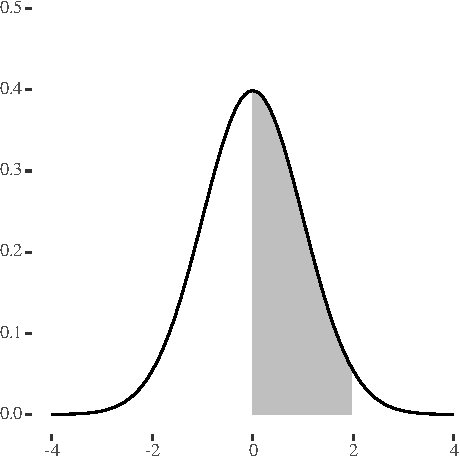
\includegraphics{NormTable_files/figure-latex/unnamed-chunk-1-1} 

}

\caption[正規分布表で求められる面積]{正規分布表で求められる面積}\label{fig:unnamed-chunk-1}
\end{marginfigure}

 

\hypertarget{rux3067ux6c42ux3081ux308bux5834ux5408}{%
\section{\texorpdfstring{\textbf{Rで求める場合}}{Rで求める場合}}\label{rux3067ux6c42ux3081ux308bux5834ux5408}}

 \textbf{R}で\(Z\)スコアから正規分布の面積を求める場合は\texttt{pnorm()}関数、面積から\(Z\)スコアを求めるには\texttt{qnorm()}関数がありますが、引数の指定には注意が必要です。例えば面積が\(95\%\)になる、すなわち約\(\pm2\sigma\)の範囲になる面積から\(Z\)スコアを求めようとして、以下のように指定した場合

\begin{Shaded}
\begin{Highlighting}[numbers=left,,]
\FunctionTok{qnorm}\NormalTok{(}\FloatTok{0.95}\NormalTok{)}
\end{Highlighting}
\end{Shaded}

\begin{verbatim}
## [1] 1.644854
\end{verbatim}

求められた\(Z\)スコアは明らかに約\(\pm1\sigma\)の面積に相当する\(Z\)スコアになっています。これは、\texttt{qnorm()}関数が下側(\texttt{-Inf})から計算して面積が\(95\%\)になる\(Z\)スコア、つまり、正規分布表で面積が\(90\%\)になる\(Z\)スコアを求めているためです。

\begin{marginfigure}

{\centering 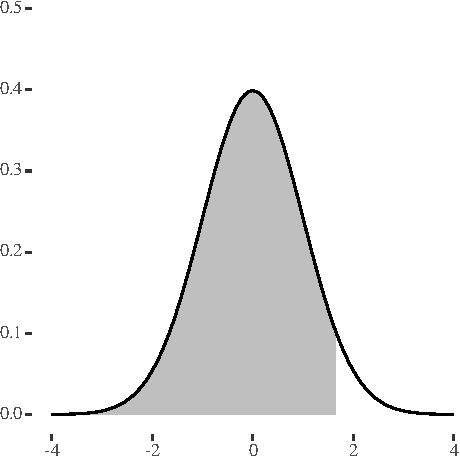
\includegraphics{NormTable_files/figure-latex/unnamed-chunk-3-1} 

}

\caption[関数が求めている面積]{関数が求めている面積}\label{fig:unnamed-chunk-3}
\end{marginfigure}

 

そこで、\texttt{qnorm()}関数で正規分布表と同じ計算を行うためには両側で\(95\%\)、つまり片側が\(\frac{1 - 0.95}{2} = 0.025\)が上側(\texttt{Inf})からの面積となる\(Z\)スコアを求める必要があります。

\begin{marginfigure}

{\centering 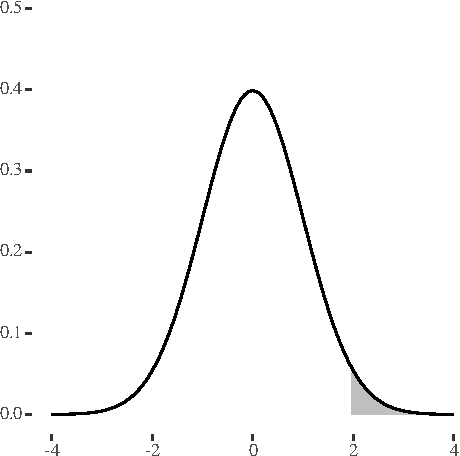
\includegraphics{NormTable_files/figure-latex/unnamed-chunk-4-1} 

}

\caption[上側$2.5\%$の面積を指定した場合]{上側$2.5\%$の面積を指定した場合}\label{fig:unnamed-chunk-4}
\end{marginfigure}

\begin{Shaded}
\begin{Highlighting}[numbers=left,,]
\FunctionTok{qnorm}\NormalTok{((}\DecValTok{1} \SpecialCharTok{{-}} \FloatTok{0.95}\NormalTok{) }\SpecialCharTok{/} \DecValTok{2}\NormalTok{, }\AttributeTok{lower.tail =} \ConstantTok{FALSE}\NormalTok{)}
\end{Highlighting}
\end{Shaded}

\begin{verbatim}
## [1] 1.959964
\end{verbatim}

同様に\(90\%\)であれば

\begin{Shaded}
\begin{Highlighting}[numbers=left,,]
\FunctionTok{qnorm}\NormalTok{((}\DecValTok{1} \SpecialCharTok{{-}} \FloatTok{0.90}\NormalTok{) }\SpecialCharTok{/} \DecValTok{2}\NormalTok{, }\AttributeTok{lower.tail =} \ConstantTok{FALSE}\NormalTok{)}
\end{Highlighting}
\end{Shaded}

\begin{verbatim}
## [1] 1.644854
\end{verbatim}

\(68.3\%\)であれば

\begin{Shaded}
\begin{Highlighting}[numbers=left,,]
\FunctionTok{qnorm}\NormalTok{((}\DecValTok{1} \SpecialCharTok{{-}} \FloatTok{0.683}\NormalTok{) }\SpecialCharTok{/} \DecValTok{2}\NormalTok{, }\AttributeTok{lower.tail =} \ConstantTok{FALSE}\NormalTok{)}
\end{Highlighting}
\end{Shaded}

\begin{verbatim}
## [1] 1.000642
\end{verbatim}

となります。

 

一方、\texttt{pnorm()}関数は\(Z\)スコアから正規分布の面積を求める関数で\texttt{qnorm()}と同様の考え方で計算しますので、\(Z\)スコアが\(1.0, 1.65, 1.96\)の場合、その上側の片側面積は

\begin{Shaded}
\begin{Highlighting}[numbers=left,,]
\FunctionTok{pnorm}\NormalTok{(}\FunctionTok{c}\NormalTok{(}\FloatTok{1.00}\NormalTok{, }\FloatTok{1.65}\NormalTok{, }\FloatTok{1.96}\NormalTok{), }\AttributeTok{lower.tail =} \ConstantTok{FALSE}\NormalTok{)}
\end{Highlighting}
\end{Shaded}

\begin{verbatim}
## [1] 0.15865525 0.04947147 0.02499790
\end{verbatim}

となります。両側面積は片側の\(50\%\)から上記を引いたものを倍にすれば良いことがわかります。

\begin{Shaded}
\begin{Highlighting}[numbers=left,,]
\NormalTok{(}\FunctionTok{pnorm}\NormalTok{(}\DecValTok{0}\NormalTok{) }\SpecialCharTok{{-}} \FunctionTok{pnorm}\NormalTok{(}\FunctionTok{c}\NormalTok{(}\FloatTok{1.00}\NormalTok{, }\FloatTok{1.65}\NormalTok{, }\FloatTok{1.96}\NormalTok{), }\AttributeTok{lower.tail =} \ConstantTok{FALSE}\NormalTok{)) }\SpecialCharTok{*} \DecValTok{2}
\end{Highlighting}
\end{Shaded}

\begin{verbatim}
## [1] 0.6826895 0.9010571 0.9500042
\end{verbatim}

 

\hypertarget{ux307eux3068ux3081}{%
\section{まとめ}\label{ux307eux3068ux3081}}

 \texttt{qnorm()}関数を用いる場合は正規分布表とは逆に上限(\texttt{Inf})側からの値を指定、\texttt{pnorm()}関数を用いる場合は求められた値を\(0.5\)から引いたものを\(2\)倍することで、正規分布表と同等の値を得ることができます。

 

\hypertarget{ux554fux984c}{%
\subsection{問題}\label{ux554fux984c}}

 \texttt{pnorm()}関数を用いて正規分布表を作成しなさい。

 

\hypertarget{about-handout-style}{%
\section{About handout style}\label{about-handout-style}}

The Tufte handout style is a style that Edward Tufte uses in his books
and handouts. Tufte's style is known for its extensive use of sidenotes,
tight integration of graphics with text, and well-set typography. This
style has been implemented in LaTeX and HTML/CSS\footnote{See Github
  repositories
  \href{https://github.com/tufte-latex/tufte-latex}{tufte-latex} and
  \href{https://github.com/edwardtufte/tufte-css}{tufte-css}},
respectively.

 

\bibliography{bib/references.bib}



\end{document}
